% !TEX root = ms.tex
\chapter{Arquitectura Software}

En el presente capítulo se describe la arquitectura software empleada para la
implementación de la MCE. Es importante resaltar que dicha arquitectura debe
coordinar y optimizar múltiples componentes que interactúan entre sí, donde la forma 
en la que se integran estos componentes impacta directamente en la
capacidad de la MCE para resolver problemas de manera eficiente y efectiva. Por
ello, en este capítulo se presenta una arquitectura modular que facilita la
experimentación y el reemplazo de componentes sin afectar al resto del sistema.
Gracias a esta modularidad, el capítulo de experimentación podrá evaluar
distintas aproximaciones cognitivas para la MCE sin necesidad de desarrollar un
sistema independiente para cada una de ellas.

Con el fin de simplificar la lectura de los capítulos posteriores, a partir de
ahora se entenderá por \emph{MCE} a la arquitectura software descrita en este capítulo.
Cuando se haga referencia al fundamento teórico de la MCE, se empleará el término
\emph{modelo teórico} de la MCE.

\section{Capas y Módulos de la MCE}

La MCE desarrollada está compuesta por cuatro módulos principales, cada uno
directamente relacionado con las entidades definidas en el modelo teórico de la
MCE. Estos módulos son:

\begin{itemize}

    \item \textbf{Capa de Cognición}: Este módulo contiene la lógica cognitiva
    de la MCE. Aquí se integran los algoritmos de percepción, aprendizaje,
    comportamiento, planificación y razonamiento de los agentes de la MCE. Cada
    agente utiliza la información obtenida de las demás capas para tomar
    decisiones e interactuar con su entorno de forma específica. No obstante,
    todos ellos comparten la dependencia de uno o varios modelos de lenguaje
    para la toma de decisiones.
    
    Esta capa se corresponde directamente con la función de cognición del modelo 
    teórico de la MCE, donde la base de
    conocimiento \(\mathbb{C}^*\) equivale a la información extraída de los LLMs y
    el mapa de correspondencia \(\Lambda\) resulta de la conversión de dicho
    razonamiento en tokens que, posteriormente, serán procesados por la Capa de
    Ejecución.

    \item \textbf{Capa de Ejecución}: Este módulo es el responsable de traducir
    los tokens generados por la Capa de Cognición en un conjunto de acciones que
    la MCE ejecutará. En capítulos posteriores se describirá este proceso como
    “interpretación” del plan generado por la LLM. Más allá de una simple
    concatenación de acciones, la Capa de Ejecución gestiona la creación de
    procesos, la desambiguación de tokens, la paralelización, la trazabilidad y
    la gestión de errores a nivel software. 
    
    Al igual que la Capa de Cognición,
    esta capa se relaciona directamente con la función de ejecución del modelo
    teórico de la MCE, al traducir tokens \(\Lambda\) en acciones pertenecientes
    al espacio \(\mathbb{B}^*\).

    \item \textbf{Espacio de Acciones}: Este módulo contiene el conjunto finito
    de acciones que la MCE puede ejecutar. Incluye tanto las acciones
    elementales del espacio \(\mathbb{B}\) del modelo teórico de la MCE como un
    conjunto creciente de acciones correspondientes al aproximador
    \(\mathbb{A}^*\). Entre las acciones elementales se encuentran mecanismos
    para la percepción de elementos en pantalla e interacción con el entorno vía
    mouse o teclado, mientras que las acciones de \(\mathbb{A}^*\) abarcan
    operaciones de alto nivel e integración con APIs del sistema operativo. 

    Como se detallará más adelante, la MCE puede dividirse en dos máquinas: una
    máquina maestra que ejecuta todas las capas de la MCE y una máquina esclava
    que realiza las acciones recibidas del maestro. Por esta razón, el Espacio
    de Acciones es compatible con diversos sistemas operativos (por ejemplo,
    Windows, Linux/Ubuntu o Raspbian), de modo que cualquiera de ellos puede
    actuar como esclavo de una MCE remota.

    \item \textbf{Capa Núcleo}: Este módulo se encarga de orquestar y coordinar
    todos los módulos de la MCE, además de construir los recursos necesarios
    para su funcionamiento. A diferencia de los demás módulos, la Capa Núcleo no
    está diseñada para ser reemplazada ni forma parte del modelo teórico de la
    MCE. En cambio, su función es aprovechar las capacidades de las demás capas
    para ejecutar la MCE, ya sea de forma local o remota.

\end{itemize}

Adicionalmente a estos módulos, la MCE incluye un conjunto de herramientas
como el registro de entidades, instaladores o manejadores del sistema que ayudan
en la coordinación de todos las capas y módulos. 

En las siguientes secciones se describirá con mayor detalle cada uno de los módulos
y herramientas de la MCE. La descripción se realizará comenzando desde las interacciones
a más bajo nivel, es decir, desde el propio espacio de acciones, y se irán conformando
abstracciones de alto nivel a medida que nos acercamos a las capas de cognición.

\section{Espacio de Acciones}

Dentro de esta capa debemos integrar acciones que satisfagan las propiedades
definidas en el espacio de acciones \(\mathbb{B}^*\) del modelo teórico de la
MCE.Todas estas acciones serán ejecutadas en la máquina controlada, a la que
denominaremos como máquina esclava. Estas acciones se dividen en dos grupos,
el espacio de acciones elementales \(\mathbb{B}\) y el espacio de acciones
\(\mathbb{A}^*\). 

A su vez, el espacio de acciones también puede ser categorizado en 3 distintas categorías:

\begin{itemize}

    \item \textbf{Acciones actuadoras}: Son aquellas que interactuan con el entorno en el
    se encuentra la máquina controlada. Estas permiten al agente cambiar el estado actual
    y la composición de este tipo de acciones permite alcanzar el objetivo final.

    \item \textbf{Acciones perceptivas}: Son aquellas que permiten al agente obtener 
    información de su entorno. Estas acciones son fundamentales para la toma de decisiones,
    pues no será posible alcanzar muchos objetivos sin previamente conocer el estado actual
    de la máquina esclava.

    \item \textbf{Meta-Acciones}: Son aquellas que permiten al agente modificarse a si mismo,
    ya sea para guardar razonamientos en memoria, para activar distintos modos de razonamiento
    o para cambiar el estado del agente. Esto permite al agente adapatarse a entornos cambiantes.

\end{itemize}

\subsection{Acciones Elementales}

Aunque el espacio de acciones \(\mathbb{B}\) puede ser ampliado con
el tiempo, a continuación se realizará un resumen de la implementación de las acciones más fundamentales para una
MCE en el entorno de un escritorio clásico. Estas son, el control del teclado,
la captura de pantalla y el control del mouse.

\subsubsection{Control del Teclado}

Las acciones de control del teclado son sencillas de implementar dadas las librerías
\texttt{pyautogui} y \texttt{uinput} de Python. En el primero caso la función 
\texttt{write()} de \texttt{pytautogui} realiza la escritura de un texto dado de forma automática.

En el caso de usar un sistema operativo Linux o Raspbian, la librería \texttt{uinput} nos
ofrece un control mas granular sobre los eventos del teclado, donde \texttt{pyautogui} puede fallar
debido a problemas de incompatiibilidad o permisos con distintas distribciones de Linux. 
En este caso, resulta necesario realizar un remapeo entre las los posibles eventos de teclado
(\texttt{uinput.KEY\_A}, \texttt{uinput.KEY\_MINUS}, etc.) y los caracteres de la cadena de 
texto objetivo a escribir (\texttt{'a'}, \texttt{'-'}, etc.).

Esta funcionalidad, se envolverá dentro de una función unica para todos los sistemas operativos, 
y permitira al agente escribir texto en la máquina esclava de forma autónoma:

\begin{lstlisting}[caption={Control del teclado}, label={cod:write_example}]
>> write("Este texto sera escrito usando el teclado")
>> Este texto sera escrito usando el teclado
\end{lstlisting}

Un caso de uso un poco más complejo es el de utilizar combinaciones de teclas
o atajos de teclado. En este caso, podemos utilizar las funciones de \texttt{pyautogui}
o \texttt{uinput} para enviar una secuencia de teclas, sin embargo, necesitamos definir
un estándar para la representación de estas combinaciones. Para resolver esto, se
ha creado un diccionario de combinaciones de teclas que incluyen multiples represntaciones
de una misma combinacion o tecla, como puede ser \texttt{CTRL}, \texttt{CONTROL} o \texttt{CTRL\_LEFT}.
De esta forma el agente podría utilizar la siguiente sintaxis:

\begin{lstlisting}[caption={Control del teclado con combinaciones de teclas}, label={cod:write_combination_example}]
>> press("CTRL + C")
KeyboardInterrupt
\end{lstlisting}

Estos dos tipos de acciones, entran en la categoría de acciones actuadoras y pertenecen al 
espacio de acciones elementales \(\mathbb{B}\). Esto se debe a que multiples aplicaciones 
no pueden ser controladas sin la capacidad de escribir texto o enviar combinaciones de teclas.

\subsubsection{Captura de Pantalla}
La captura de pantalla es una de las acciones perceptivas que más información
brinda sobre el estado actual de la máquina esclava. Sin embargo, a su vez esta
información tiene el coste computacional más alto, ya que requiere tanto un 
preprocesamiento de la imagen como un análisis posterior para extraer la información
necesaria.

Para la captura de pantalla se utiliza la librería \texttt{pyautogui}, que 
atravesará por varios modulos de OCR (Reconocimiento Óptico de Caracteres),
algoritmos de detección de elementos (creados con \texttt{OpenCV})\footnote{Adicionalmente para eliminar los falsos positivos, se utiliza una métrica basada en Iou (Intersection over Union)}
y modelos multimodales basados en LLM para extraer tanto las entidades visuales como
textuales de la imagen capturada. Una vez procesada la imagen, se puede 
generar una representación de la misma mediante un conjunto de bounding
boxes que indican la posición de los elementos detectados y que, posteriormente,
será utilizada para la toma de decisiones.

\begin{figure}[!h]
	\centering
	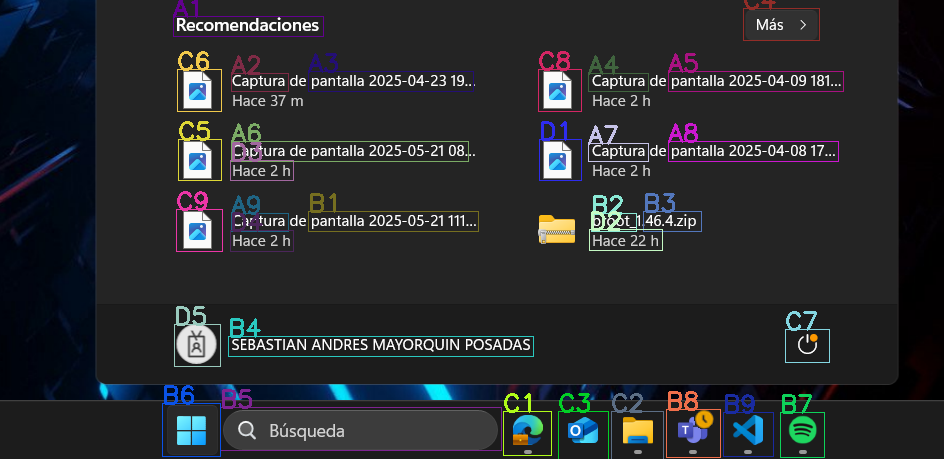
\includegraphics[scale=0.3]{figs/ocr_image.png}
	\caption{\small Procesamiento de una captura de pantalla con algoritmos de detección de elementos. Fuente: Elaboración Propia.}
	\label{fig:ocr_image}
\end{figure}

Notese que aunque esta acción es perceptiva, tambien forma parte de las acciones
elementales \(\mathbb{B}\) del espacio de acciones, ya que multiples 
problemas no pueden ser resueltos sin distinguir los elementos presentes
de forma visual, como por ejemplo, la interfaz gráfica de un videojuego.

\subsubsection{Control del Mouse}

El control del mouse es una acción actuadora y elemental que permite al agente interactuar
con la interfaz gráfica de la máquina esclava. Para llevarla a cabo, se puede
utilizar la librería \texttt{pyautogui} tanto en Windows como en Raspbian.

En sistemas Linux sin embargo, es importante considerar el tipo de entorno
gráfico utilizado. En entornos basados en X11, los permisos para controlar el
mouse son relativamente permisivos. En cambio en sistemas que utilizan Wayland,
por motivos de seguridad, los eventos del mouse solo pueden enviarse a la ventana que esté activa
originalmente.

Esto significa que, si el agente intenta controlar una ventana distinta, el
movimiento del mouse quedará bloqueado hasta que el usuario vuelva a activar
manualmente la ventana original.

Estos problemas de compatibilidad se pueden resolver utilizando herramientas
como \texttt{ydotool} o bien realizando una calibración previa de la sensibilidad 
del mouse y usando \texttt{uinput} para enviar eventos de mouse.

Una vez resueltos estos problemas, el agente podrá interactuar con la máquina
tal que:

\begin{lstlisting}[caption={Control del mouse}, label={cod:mouse_example}]
>> move_mouse(100, 200)
>> double_click()
>> move_mouse(300, 400)
>> right_click()
\end{lstlisting}

\subsection{Espacio de Acciones \(\mathbb{A}^*\)}
El espacio de acciones \(\mathbb{A}^*\) es infinito por definición. En el caso 
de la arquitectura implementada se han desarrollado alrededor de 20 paquetes 
de acciones, donde cada uno de estos paquetes contiene entre 1 y 3 acciones
dependiendo de la complejidad del problema a resolver.

A continuación se describen algunas de las acciones más relevantes
del espacio de acciones \(\mathbb{A}^*\):

\subsubsection{Espera Condicional}
La espera condicional o \texttt{wait\_for()} es una meta-acción que permite al agente
esperar hasta que se cumpla una determinada condición antes de continuar con la
ejecución de la siguiente acción. Esta acción permite ahorrar una gran parte de los
recursos computacionales gastados mientras un elemento se carga o una ventana se abre.

Para dejar al agente bloqueado, bastará con utilizar la función \texttt{sleep()}
de Python, sin embargo la detección de la condición a esperar es una tarea más
sensible y compleja. Para ello, se utiliza un modelo multimodal que es capaz de
recibir una condición dada en lenguaje natural, y analizará periodicamente
la pantalla para determinar si la condición se ha cumplido o no.

Como ejemplo, el agente podría esperar a que aparezca un botón de
\texttt{Aceptar} en la pantalla tal que:

Es importante tener en cuenta los casos en los que la condición nunca se
cumple, ya que esto podría bloquear al agente indefinidamente. Para evitarlo,
el propio agente puede establecer un tiempo máximo de espera, tras el cual
se cancelará la espera y se continuará con la ejecución del programa.

\begin{lstlisting}[caption={Espera condicional}, label={cod:wait_for}]
>> wait_for("Aparicion del boton 'Aceptar'", timeout=30)
Esperando a que aparezca el boton Aceptar...
Esperando a que aparezca el boton Aceptar...
Esperando a que aparezca el boton Aceptar...
Condicion cumplida: El boton Aceptar ha aparecido en la pantalla.
>> 
\end{lstlisting}

\subsubsection{Abrir Aplicación}
La acción de abrir una aplicación es una de las más comunes y útiles para
la MCE, pues una gran parte de los problemas a resolver requieren la
interacción con aplicaciones específicas. Así pues esta acción permite traducir
lenguaje natural a una busqueda de aplicaciones en el sistema operativo esclavo.

Para realizar esto, se realiza una busqueda en múltiples directorios con usualmente
utilizados como directorios de instalación de aplicaciones, como por ejemplo, \texttt{/usr/bin} en
el caso de Linux o \texttt{C:\textbackslash Program Files} en el caso de Windows; y se
utiliza un algoritmo de similitud de cadenas para encontrar la aplicación más
similar al nombre de la aplicación proporcionado por el agente.

Gracias a esta acción, el agente puede abrir e interactuar con aplicaciones tal que:

\begin{lstlisting}[caption={Abrir aplicación Spotify}, label={cod:open_application}]
>> open_application("Spotify")
Abriendo Spotify...
>>
\end{lstlisting}

Nótese que aunque esta acción puede ser completada unicamente mediante acciones elementales
(clicks y escritura de texto), su implementación permite una interacción mas agil y eficiente
con el sistema. Formalmente, reeemplazamos una solucion \(s_{sub}\) con una solución \(s_{opt}\)
ambas pertenecientes a \(\mathbb{S}_p\)

\subsubsection{Ejecución de Código}
La acción de ejecución de código permite al agente ejecutar código Python, JavaScript, bash
o powershell en la máquina esclava. Esta acción tiene optimiza especialmente
las tareas de gestión y/o modificación de archivos, ya que permite al agente
realizar operaciones complejas de forma rápida y eficiente.

Sin embargo, es importante tener en cuenta que esta acción puede ser peligrosa si
el agente no esta debidamente controlado, es por ello que se ha implementado 
adicionalmente una interfaz gráfica de seguridad que mantiene al usuario informado
del código que se está ejecutando y le permite garantizar o denegar la ejecución
de la acción en cualquier momento.

\begin{figure}[!b]
	\centering
	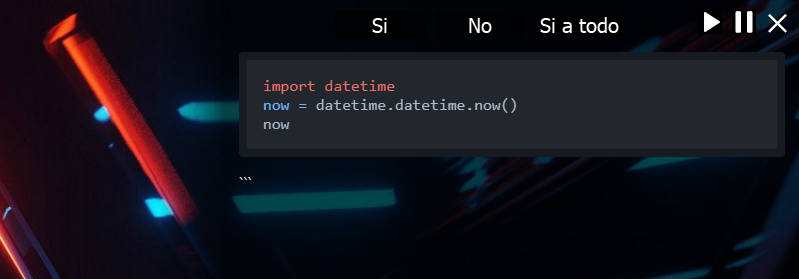
\includegraphics[scale=0.4]{figs/code_execution.png}
	\caption{\small Interfaz gráfica de seguridad para ejecución de código. Elaboración Propia}
	\label{fig:code_execution}
\end{figure}

\section{Capa de Ejecución}

Como se ha descrito en secciones anteriores, la capa de ejecución es
la encargada de traducir los tokens generados por la capa de cognición en
acciones que la MCE ejecutará en la máquina esclava. 

Este proceso de ejecución utiliza 2 componentes principales: 

\begin{itemize}

    \item \textbf{Exelent}: Exelent es un lenguaje declarativo de alto nivel 
    concebido y diseñado en este proyecto para ser utilizado por modelos de lenguaje. 
    Este lenguaje viene junto a un mecanismo de procesamiento que tokeniza/compila este 
    lenguaje y lo convierte en una representación que puede ser entendida por un intérprete.

    \item \textbf{Intérprete}: El intérprete es el componente encargado de
    enlazar los tokens generados por la capa de Cognición con las acciones
    correspondientes en el espacio de acciones \(\mathbb{B}^*\). A su vez, el
    intérprete convierte los tokens en "tareas" que pueden ser ejecutadas.
    Estas tareas siempre se asegura que estan definidas siguiendo el protocolo
    TSP (Task-Sequence Protocol), que define el conjunto de reglas que ambos
    componentes deben seguir para garantizar la correcta sincronización de los 
    componentes.
    
\end{itemize}

A continuación se describen con más detalle los mecanismos internos de cada uno
de estos componente y su funcionamiento en la capa de ejecución.

\subsection{Task-Sequence Protocol (TSP)}

El protocolo TSP es un conjunto de reglas que define cómo deben ejecutarse
las acciones en la MCE. Este protocolo contiene una estructura de 3 niveles 
que permite organizar las acciones de forma jerárquica. 

Estos 3 niveles son:

\begin{itemize}

    \item \textbf{Acción}: Una acción es la unidad más básica de ejecución en
    el protocolo TSP. Cada acción representa una única acción correspondiente al
    espacio de acciones \(\mathbb{B}^*\). Puesto que todas las acciones se representan
    a su vez mediante una única funcion Python, cada acción estará compuesta por
    un nombre de la acción y un conjunto de argumentos que serán utilizados por la
    función correspondiente.

    \item \textbf{Secuencia}: Una secuencia es un elemento que agrupa acciones
    y/o otras secuencias y define un mecanismo de ejecución. Este mecanismo
    puede ser secuencial, paralelo, condicional, iterativo, etc. Las secuencias y/o 
    acciones serán ejecutadas siguiendo el mecanismo definido por la secuencia. Esto 
    permite al agente combinar acciones de forma flexible y adaptativa.

    \item \textbf{Tarea}: Una tarea es el elemento más alto del protocolo TSP y
    representa una unidad de trabajo que puede ser ejecutada por la MCE. Una tarea
    puede (de forma opcional) contener una prioridad, un identificador y modificadores
    de control. 
    
    La prioridad permite al agente crear situaciones en las que ciertas
    acciones deben ser ejecutadas interrumpiendo otras acciones en curso; por ejemplo,
    un agente puede decidir parar un ánalisis si recibe una notificación de un
    evento importante.
    
    El identificador es generado automaticamente por el intérprete y permite a
    la capa de ejecución mantener un registro de las tareas en curso. 

    Los modificadores de control permiten al agente definir condiciones de ejecución como
    "esta tarea debe ejecutarse solo si la tarea anterior ha finalizado con éxito". 
    Estos modificadores son especialmente útiles para la creación de tareas
    complejas que requieren de una ejecución controlada y secuencial.

\end{itemize}

En el caso del lenguaje exelent, este esta estructurado de forma que todas las tareas
contienen los tres niveles del protocolo TSP. A su vez, el intérprete debe ser capaz
de convertir cualquier tarea que siga el protocolo TSP en código ejecutable por la MCE.

\subsection{Exelent}
Exelent (haciendo referencia al juego de palabras "Exe-cution Lan-guage") es un
lenguaje declarativo que permite a los modelos de lenguaje escribir acciones
siguiendo el protocolo TSP utilizando lenguaje natural. A su vez, este lenguaje
esta diseñado para poder ser generado por LLMs sin necesidad de realizar
fine-tunning o entrenamiento adicional. Esto se debe a su sencillez de
estructura y gramática lo que permite su utilización con distintos modelos de
forma efectiva.


A modo de ejemplo conceptual, se presenta a continuación un fragmento de
pseudocódigo que representa la lógica general de exelent sin exponer
detalles de implementación concretos:

\begin{lstlisting}[caption={Fragmento de pseudocódigo Exelent}, label={cod:exelent_example}]
>> start opening firefox with priority normal
>>   parallel run
>>     open_application "Firefox"
>>     wait_for "Firefox is ready"
>>
>>   on exit
>>     if "Firefox is not ready" then
>>       replan "Firefox failed to open"
>>     else
>>       complete "Firefox opened successfully"
>>     end if
>>
>>   on error
>>     replan "An error occurred while opening Firefox"
>>
\end{lstlisting}

En este ejemplo, el agente inicia la apertura de Firefox con una prioridad 
normal. Dentro de esta tarea, vemos como distintos tipos de secuancia permiten
definir la lógica de ejecución. Por ejemplo, la secuencia \texttt{parallel run} permite
ejecutar dos acciones de forma simultánea. A su vez estas secuencias contienen 
acciones que se ejecutarán siguiendo el protocolo TSP.

Para poder tokenizar este lenguaje, se ha desarrollado un tokenizador que 
convierte cada linea de código en estructuras de datos que serán utilizados 
por el intérprete. A continuación, se muestra una tokenización hipotética del
código, útil para entender la estructura del formato.

\begin{lstlisting}[caption={Ejemplo de tokenización en Exelent}, label={cod:exelent_tokenization}]
>> {
>>   "task": {
>>     "name": "opening firefox",
>>     "priority": "normal",
>>     "sequences": [
>>       {
>>         "type": "parallel",
>>         "actions": [
>>           {
>>             "action": "open_application",
>>             "args": ["Firefox"]
>>           },
>>           {
>>             "action": "wait_for",
>>             "args": ["Firefox is ready"]
>>           }
>>         ]
>>       }
>>     ],
>>     "on_exit": {
>>       "if": {
>>         "condition": "Firefox is not ready",
>>         "then": {
>>           "action": "replan",
>>           "args": ["Firefox failed to open"]
>>         },
>>         "else": {
>>           "action": "complete",
>>           "args": ["Firefox opened successfully"]
>>         }
>>       }
>>     },
>>     "on_error": {
>>       "action": "replan",
>>       "args": ["An error occurred while opening Firefox"]
>>     }
>>   }
>> }
\end{lstlisting}

\subsection{Intérprete}
El intérprete es el componente encargado de procesar los tokens generados desde
el lenguaje exelent tokenizado y crear una estructura de datos ejecutable que
cumpla las condiciones del protocolo TSP. A su vez el intérprete es el encargado
de enlazar las acciones con las funciones correspondientes del espacio de
acciones \(\mathbb{B}^*\).

En este proyecto se han implementado dos intérpretes distintos\footnote{
Nótese que la naturaleza modular de la MCE permite que el intérprete pueda ser
reemplazado por cualquier otro intérprete que cumpla las condiciones del
protocolo TSP.}, uno basado en servicios del framework ROS2 (denominado como
ROSA) que permitió la creación de un prototipo funcional y depurable; y otro
creado puramente en Python (denominado como Pyxcel, del juego de palabrras
"Py-thon E-xcel-ent") que realiza enlaza las acciones \emph{just-in-time}, es
decir, cargando los módulos necesarios únicamente cuando son necesarios.


Pyxcel es un intérprete mas eficiente, ligero y modular que ROSA, eliminando complejidades
innecesarias (debido principalmente a la naturaleza modular de ROS2) y permitiendo
una integración más sencilla con el resto de la MCE.

Para realizar el enlace de las acciones, el intérprete consulta un mecanismo global
de la MCE denominado como \texttt{ItemRegistry} o \emph{Registro de Entidades}. 
Este registro (que será descrito en más profundidad en secciones posteriores) contiene una 
base de datos de todas las acciones disponibles en el espacio de acciones \(\mathbb{B}^*\) y
el codigo Python correspondiente a cada una de ellas. De esta forma, el intérprete
consulta el registro para obtener todas las acciones similares a la acción solicitada y
realiza un proceso de desambiguación para seleccionar la acción más adecuada.

Una vez se ha seleccionado la acción, el intérprete crea un proceso paralelo y vigila 
su ejecución. Esta acción puede a su vez generar fragmentos de retroalimentación que 
recibidos por el intérprete, serán procesados y enviados a la capa de cognición. Mientras
la ejecución se encuentra en curso, el intérprete también puede recibir nuevos eventos
desde la capa de cognición, donde el intérprete puede decidir si continuar con la ejecución,
mandar señales de parada, cancelación o realizar un envío de recursos adicionales.

Gracias a este mecanismo, el resto de capas de la MCE pueden utilizar lenguaje Exelent para
poner en marcha la ejecución de una tarea, sin necesidad de preocuparse por los detalles
de control o implementación de cada acción.

\section{Capa de Cognición}

La capa de cognición es el conjunto de componentes que permiten dotar de 
"inteligencia" cognitiva a la MCE. Formalmente, esta capa se corresponde 
con la función de cognición del modelo teórico de la MCE. Nótese que en esta capa
asumiremos que la base de conocimiento \(\mathbb{C}\) es un modelo de lenguaje
natural.

Así pues esta capa contiene tanto un kit de herramientas agénticas que dotarán
al sistema de capacidades cognitivas, como un conjunto de agentes que,
utilizando estas herramientas, serán capaces de integrarse en la MCE y consecuentemente, 
resolver problemas de forma autónoma.

En este capítulo se describirán algunos de los mecanismos internos más 
relevantes de la capa de cognición independientemente de los agentes que los utilicen. Estos agentes serán
descritos en el capítulo de experimentación, donde se presentarán distintas
aproximaciones cognitivas para la MCE.

\subsection{Autodescriptor de Acciones}
Para que un agente pueda utilizar el espacio de acciones \(\mathbb{B}^*\) de la 
MCE, es necesario que se cumplan las siguientes condiciones:


\begin{enumerate}
    \item El agente debe ser previamente informado de las acciones 
    disponibles en el espacio de acciones \(\mathbb{B}^*\).

    \item El agente debe ser informado de los requisitos o entradas de cada
    una de las acciones disponibles en el espacio de acciones, así como de los
    posibles resultados o salidas de cada una de ellas.

    \item El agente debe conocer un formato de representación adecuado para poder
    utilizar el espacio de acciones de forma efectiva.
\end{enumerate}

Para resolver estos 3 problemas, se ha desarrollado un mecanismo denominado como
\emph{Autodescriptor de Acciones}. Este mecanismo permite generar una descripción
automática de las acciones disponibles en el espacio de acciones \(\mathbb{B}^*\) de la MCE.


\begin{itemize}
    \item \textbf{Autoformato}: El autodescriptor utiliza el \emph{registro de entidades} de la 
    MCE para obtener todas las acciones disponibles en el espacio de acciones. Para cada una de ellas
    utiliza un formato json que contiene el nombre de la acción, una breve descripción de su caso de uso,
    los argumentos necesarios para su ejecución y una breve descripción de los posibles resultados.

    \item \textbf{Mapa de Correspondencia}: Para cada una de las acciones, el autodescriptor enlaza
    el nombre de la acción con un conjunto de sinónimos y términos relacionados. Todos estos términos
    son correlacionados con la acción y se almacenarán en el mapa de correspondencia \(\Lambda\) utilizado
    en la capa de ejecución. De esta forma, cuando el agente solicite una acción, la capa de cognición
    podrá buscar en el mapa de correspondencia \(\Lambda\) y generar codigo exelent que
    pueda ser ejecutado por la capa de ejecución.

    A su vez el autodescriptor también genera un set de instrucciones que
    pueden ser utilizadas por el agente para comprender cómo utilizar el espacio 
    de acciones \(\mathbb{B}^*\) de la MCE.

\end{itemize}


Como ejemplo ilustrativo, supongamos un espacio de acciones conformado exclusivamente por
la acción de control de teclado \texttt{write()}. El autodescriptor generaría
la siguiente descripción:

\begin{lstlisting}[caption={Autodescriptor de acciones}, label={cod:autodescriptor_example}]
>> {
>>   "name": "write",
>>   "description":
>>     "Escribe un texto dado en la maquina esclava.",
>>   "args": {
>>     "text":
>>       "El texto a escribir.
>>   },
>>   "returns": {
>>     "success":
>>       "Indica si la escritura fue exitosa."
>>   }
>> }
\end{lstlisting}


A su vez, el mapa de correspondencia \(\Lambda\) sería actualizado tal que:
\begin{lstlisting}[caption={Mapa de correspondencia}, label={cod:correspondence_map_example}]
>> {
>>     "write": [
>>         "write",
>>         "escribir",
>>         "introducir texto",
>>         "input"
>>     ]
>> }
\end{lstlisting}
De esta forma, el agente puede utilizar el espacio de acciones \(\mathbb{B}^*\) de la MCE
de forma efectiva, generando código exelent siguiendo las instrucciones embedidas en el autodescriptor.

\begin{lstlisting}[caption={Ejemplo de uso del autodescriptor}, label={cod:autodescriptor_usage_example}]
>> agent.invoke("Por favor escribe 'Hola Mundo' en la maquina esclava")
>> Resultado: 
>> ```
>> start writing hello world with priority normal
>>     sequentially run
>>         write "Hello World"
>> ```

\end{lstlisting}

Posteriormente, este fragmento de código sería enviado a la capa de ejecución
para ser procesado por el intérprete y ejecutado en la máquina esclava.

Gracias a este mecanismo los agentes de la MCE podrán utilizar el espacio de
acciones \(\mathbb{B}^*\) de forma efectiva, sin necesidad de preocuparse por los
detalles de la implementación.

\subsection{Buffer de Memoria}
Siguiendo la arquitectura PMPA discutida en la sección \ref{sec:components_of_cognitive_architectures}
la MCE implementa un buffer de memoria que permite a los agentes mantener coherencia
a lo largo de la ejecución de una tarea. 

En su forma más básica, una memoria no es más que un vector de mensajes que 
contienen tanto la entrada del usuario, como información del entorno,
y los resultados de las acciones realizadas por el agente. Sin embargo,
a nivel práctico la memoria debe contener únicamente la información relevante
que el agente necesita para tomar decisiones y resolver problemas.

Para ello, la MCE implementa un buffer de memoria que en cada actualización
realiza un análisis de la información almacenada, eliminando la información 
redundante, de gran volumen, o que no es relevante para la tarea en curso.

Como ejemplo ilustrativo, supongamos que un agente ha recibido la siguiente
información en su buffer de memoria:

\begin{lstlisting}[caption={Buffer de memoria}, label={cod:memory_buffer_example}]
>> [
>>     ("user", "Por favor escribe 'Hola Mundo' en la maquina esclava 
>>        y luego haz click en cerrar ventana"),
>>     ("environment", "La maquina esclava esta en el escritorio"),
>>     ("action", "start writing hello world with priority normal"),
>>     ("action", "write 'Hello World'"),
>>     ("result", "Escritura exitosa")
>> ]
\end{lstlisting}

En este caso, el buffer de memoria podría eliminar algunas entradas que
ya no son relevantes para las proximas tareas. Así, el buffer de memoria
podría actualizarse a:

\begin{lstlisting}[caption={Buffer de memoria actualizado}, label={cod:memory_buffer_updated_example}]
>> [
>>     ("user", "Por favor escribe 'Hola Mundo' en la maquina esclava 
>>        y luego haz click en cerrar ventana"),
>>     ("environment", "La maquina esclava esta en el escritorio"),
>>     ("result", "Escritura exitosa")
>> ]
\end{lstlisting}

Adicionalmente, el buffer de memoria tambíen contiene mecanismos para minimizar
el volumen de información gráfica (como capturas de pantalla) o generación automática
de resúmenes para salidas con gran volumen de texto. Con todos estos mecanismos,
los agentes mantendran un estado coherente a lo largo de la ejecución de una tarea,
sin necesidad de preocuparse por la gestión de la memoria.

\subsection{Estado Cognitivo}
El estado cognitivo es un mecanismo que permite a los agentes el uso de 
las meta-acciones. De forma simplificada, un estado cognitivo no es mas que
un conjunto de variables que definen el comportamiento que debe seguir
el agente. Cuando un agente realiza una meta-acción, esta modifica su estado cognitivo, permitiendole
influir en su propio comportamiento. 

Nótese como estas \emph{variables} en el estado cognitivo no tienen una funcionalidad específica
ni afectan en modo alguno a la MCE, sino que son utilizadas por el propio agente como indicadores 
de su comportamiento.

Como ejemplo ilustrativo, supongamos que un agente comienza una tarea 
con el siguiente estado cognitivo:

\begin{lstlisting}[caption={Ejemplo de estado cognitivo inicial}, label={cod:cognitive_state_initial_example}]
>> {
>>    "state": "normal",
>>    "short-term-goal": "None",
>>    "long-term-goal": "Play a song on Spotify"
>> }
\end{lstlisting}

En este caso, el agente podría cambiar su estado cognitivo a un modo de planificación
utilizando la siguiente meta-acción:
\begin{lstlisting}[caption={Cambio de estado cognitivo}, label={cod:cognitive_state_change_example}]
>> start thinking with priority normal
>>     parallel run
>>         set_state "planning"
>>         set_short_term_goal "Generate a plan to play a song on Spotify"
\end{lstlisting}

De este modo, el agente habría cambiado su estado cognitivo a:
\begin{lstlisting}[caption={Estado cognitivo actualizado}, label={cod:cognitive_state_updated_example}]
>> {
>>    "state": "planning",
>>    "short-term-goal": "Generate a plan to play a song on Spotify",
>>    "long-term-goal": "Play a song on Spotify"
>> }
\end{lstlisting}

Así pues, el estado cognitivo no necesita alterar directamente los mecanismos internos 
del agente, sino que su influencia se limita a modificar las instrucciones que el propio agente recibe.

De forma practica, si por ejemplo, el agente recibe un estado cognitivo que le indica que previamente
él mismo se ha asignado un objetivo a corto plazo, este seguirá su propio protocolo de ejecución
para alcanzar dicho objetivo, cambiando su estado nuevamente cuando lo considere apropiado.

El estado cognitivo a su vez, tambien puede ser programado de forma externa para 
modificarse automáticamente en función de eventos o condiciones del entorno. Por ejemplo,
un agente, podria cambiar su estado cognitivo a "razonamiento rápido" si llevara 
más de 5 minutos realizando una tarea.

Adicionalmente, una de las meta-acciones mas importantes de la MCE es la capacidad para establecer
el estado de "objetivo completado". Esta meta-acción será vigilada por la MCE para determinar si
el agente ha completado su tarea o no. Mientras que el agente no complete su objetivo, la MCE continuará
ejecutando las acciones enviadas a la capa de ejecución. Finalmente, cuando el agente complete su objetivo,
la MCE recuperará el control y decidirá si continuar con la ejecución de la tarea o finalizarla.

\subsection{Fast Agent-Protocol (FastAP)}
El protocolo FastAP esta basado en el protocolo de agentes discutido en la sección 
\ref{sec:components_of_cognitive_architectures}. En contraste con el protocolo de agentes
original, FastAP es un protocolo mucho más rápido y con una implementación sencilla que permite
embeber todas las capacidades de un agente en una única funcion de Python.

A su vez, este protocolo es totalmente síncrono y basado en un sistema de mensajes, donde
al enviar un mensaje a un agente que utiliza el protocolo FastAP, este tomára el control
de la MCE de forma temporal hasta que haya completado su tarea.

Utilizando este protocolo todos los agentes de la MCE, independientemente de su implementación
y mecanismos internos, pueden ser integrados en la MCE con una interfaz unificada.

A su vez, FastAP esta sincronizado con el resto de capas de la MCE para realizar las 
siguientes funcionalidades:

\begin{itemize}

    \item \textbf{Resolución automática de dependencias}: FastAP realiza un análisis dinámico
    de las dependencias de cada agente, tanto a nivel de librerías como a nivel de las acciones
    necesarias para cada agente. Una vez cone estas dependencias, FastAP generá un entorno virtual
    que contiene todas las dependencias necesarias para la ejecución del agente. De esta forma,
    los agentes pueden ser ejecutados sin tener conflictos con el resto de agentes o capas de la MCE.

    \item \textbf{Control de Ejecución}: FastAP permite pausar, reanudar o cancelar la ejecución
    de un agente en cualquier momento. Esto es debido, a que todos los agentes necesitan que FastAP
    envie mensajes de confirmación para continuar con la ejecución de su tarea. Cuando una señal de 
    parada es enviada, FastAP no envía más mensajes de confirmación al agente y, en caso de que una posterior
    cancelación sea enviada, FastAP eliminará el entorno virtual del agente y devolverá el control a la MCE.

    \item \textbf{Logging y Depuración}: FastAP permite registrar todas las acciones realizadas por el agente
    independiente de que este utilice acciones, meta-acciones o que llame a otros agentes. Todas esta información
    puede ser enviada a un fichero de log o a cualquier sistema de depuración que sea especificado por el sistema.

\end{itemize}

Este protocolo es un mecanismo fundamental en la MCE, pues sin el no sería posible la experimentación y contraste
de distintos agentes en la MCE. A su vez, este protocolo permite a los agentes
integrarse de forma sencilla y rápida en la MCE, pues provee de una plantilla de código
que puede ser facilmente adaptada a los mecanismos internos de cada agente.

\section{Capa de Núcleo}
La capa de núcleo tiene la responsabilidad de conectar todos los componentes
de la MCE y coordinar su funcionamiento. El modelo teórico de la MCE, no contempla
ninguna función específica para esta capa, sin embargo en la práctica, esta capa
es la que permite la correcta comunicación entre las distintas capas y componentes
de la MCE.

En este capitulo se describirán algunos de los mecanismos internos más relevantes de 
la capa de núcleo, finalmente, se presentará una visión general del funcionamiento
de la MCE.

\subsection{Registro de Entidades}
El registro de entidades es un mecanismo que permite a la MCE almacenar
todas las acciones del espacio de acciones \(\mathbb{B}^*\), sus metadatos asociados
y crear una interfaz estandarizada para que todas las capas puedan interactuar con estas acciones.

Entre las funcionalidades más relevantes del registro de entidades se encuentran:

\begin{itemize}

    \item \textbf{Resolución de Dependencias}: Mientas que FastAP se encarga de resolver
    las dependencias de los agentes, el registro de entidades se encarga de resolver
    las dependencias de las acciones. Esto incluye tanto las dependencias de librerías
    como interdependencias entre acciones. Por ejemplo, si una accion de reconocimiento de
    caracteres (OCR) depende de la librería \texttt{pytesseract}, el registro de entidades
    se encargará de asegurar que esta librería esté disponible en un entorno virtual
    que luego será utilizado por la capa de ejecución.

    \item \textbf{Carga Perezosa}: El registro permite la carga perezosa de acciones, es decir, las acciones
    no se cargan hasta que son llamadas por la capa de ejecución. Esto permite que acciones que no son utilizadas no
    consuman recursos innecesarios en el sistema. Este mecanismo resulta fundamental dado que el espacio de acciones \(\mathbb{B}^*\) 
    es teoricamente tendiente a infinito, por lo que en caso de que la carga no fuera perezosa, el sistema
    podría consumir una cantidad de recursos computacionales excesiva tanto en el inicio de la MCE como en la ejecución de las acciones.

    \item \textbf{Mapa de Correspondencia}: El registro guarda un mapa de correspondencia \(\Lambda\) basado en multiples
    diccionarios clave-valor que permiten a la capa de ejecución encontrar las acciones correspondientes a los tokens
    encontrados durante el análisis del lenguaje exelent. Debido a la carga perezosa, este mapa no apunta directamente a las funcionalidades
    de las acciones, sino que apunta a un disparador que, al ser invocado, cargará la acción en memoria y la ejecutará. En caso de 
    haber sido cargada previamente, el disparador simplemente ejecutará la acción sin necesidad de cargarla de nuevo.

    \item \textbf{Entorno Maestro-Esclavo}: El registro permite crear un entorno maestro-esclavo para dividir la ECM en dos máquinas:
    una máquina maestra que sera la encargada de ejecutar la MCE y otra esclava que ejecutará las acciones del espacio de acciones. Para
    realizar esto, el registro es capaz de modificar el disparador de las acciones para que, en lugar de ejecutar la acción directamente, 
    envíe un mensaje a la máquina esclava para que esta ejecute la acción en su lugar. A su vez, el registro evita que la acción 
    se cargue en la máquina maestra, de forma que esta no consuma recursos innecesarios.

    \item \textbf{Almacenamiento de Configuraciones}: El registro tambien permite almacenar configuraciones que pueden ser utilizadas
    por distintas capas de la MCE. De esta forma, todas las capas pueden interactuar entre sin depender de la integración de cada una de ellas.
    A su vez, también permite al cliente cambiar el comportamiento de la MCE sin necesidad de modificar el código de cada una de las capas.

    \item \textbf{Empaquetado de Acciones}: El registro permite a su vez empaquetar conjuntos de acciones en un único paquete que comparten
    funcionalidades comunes. Estos paquetes agilizan la resolucion de dependencias y a su vez permiten a los agentes simplificar la invocación 
    de acciones que generalmente son utilizadas juntas. Por ejemplo, un paquete de acciones podría contener acciones para abrir una 
    aplicación, esperar a que esta se cargue y realizar una acción específica en la aplicación, etc.

    \item \textbf{Ejecución Segura}: El registro tambíen permite a la MCE ejecutar acciones de forma segura,
    esto es el registro puede cambiar las funcionalidades de las acciones para que estas
    no se ejecuten directamente, en su lugar, pueden pedir una confirmación al usuario o bien
    ejecutar una acción simulada que no afecte al sistema. Esto es especialmente
    útil para acciones que pueden tener un impacto significativo en el sistema, como
    eliminar archivos, modificar configuraciones del sistema, etc.

\end{itemize}

\subsection{Servicio Maestro-Esclavo}
El servicio maestro-esclavo (SME) es el mecanismo encargado de gestionar las comunicaciones
entre la máquina controlada (esclava) y la máquina que ejecuta la MCE (maestra). 

Este servicio se realizó a traves de una implementación basada en RabbitMQ con
mensajes de tipo string entre ambas máquinas. Debido a la naturaleza de la MCE, 
se requiere que la ejecución de codigo en una máquina remota sea lo más segura 
posible, por lo que esta implementación ha sido reemplazada por un mecanismo 
externo basado en gRPC (Google Remote Procedure Call).

Esta implementación ha sido integrada dentro del registro de entidades, de forma
que toda la carga de acciones, metadatos y ejecución de funcionalidades sea mediante
este servicio.

\subsection{Ejemplo de Funcionamiento de la MCE}
De forma ilustrativa, el siguiente ejemplo muestra el funcionamiento
de la MCE desde el punto de vista de la capa de núcleo. En este ejemplo,
el usuario solicitará al agente que abra Spotify.

Nótese que multiples mecanismos internos han sido omitidos para
simplificar el ejemplo, a su vez, algunas simplificaciones han sido 
realizadas para facilitar la comprensión del funcionamiento de la MCE.

\begin{enumerate}
    \item El usuario arranca la MCE:
    \begin{enumerate}
        \item El registro de entidades es inicializado y se realiza una precarga 
        de todas las acciones (y metadatos) disponibles en el espacio de acciones \(\mathbb{B}^*\).
        \item El Interprete, por ejemplo Pyxcel es inicializado y se enlaza con el registro de entidades 
        y al mapa de correspondencia \(\Lambda\).
        \item Se inicializa la capa de cognición y se carga el agente integrado en 
        la MCE, por ejemplo, DarkVFR
        \item DarkVFR inicializa los modulos de la capa de cognición necesarios, como por ejemplo,
        inicializa el buffer de memoria y el estado cognitivo con los valores por defecto.
        \item FastAP es inicializado y se enlaza con la capa de cognición. Crea un entorno virtual,
        analiza las dependencias del agente, y si existen dependencias obligatorias, carga en el 
        registro de entidades las acciones necesarias.
        \item FastAP enlaza al agente (DarkVFR) con el interprete, permitiendole enviar acciones a
        la capa de ejecución.
        \item FastAP crea un servidor de control para el usuario, de forma que este pueda pararlo,
        cancelarlo o reiniciarlo en cualquier momento.
    \end{enumerate}

    \item La MCE esta lista para recibir comandos, el usuario solicita al agente que abra Spotify 
    usando el comando "Por favor abre Spotify".

    \begin{enumerate}   
        \item FastAP recibe el mensaje del usuario y lo envía a DarkVFR
        \item DarkVFR consulta el registro de entidades y utiliza el autodescriptor de acciones para generar un set
        de instrucciones para el LLM.
        \item DarkVFR guarda el mensaje en su buffer de memoria, y llama al LLM para realizar 
        una planificación.
        \item El LLM genera un plan de acción utilizando el lenguaje exelent, por ejemplo:
        \begin{lstlisting}[caption={Plan de acción generado por el LLM}, label={cod:llm_plan_example}]
>> start opening spotify with priority normal
>>     sequentially run
>>         open_application "Spotify"
        \end{lstlisting}
        \item DarkVFR envia el plan de acción a la capa de ejecución a traves del interprete.
    \end{enumerate}

    \item El interprete recibe el plan de acción y lo envia a la capa de ejecución.
    \begin{enumerate}
        \item El interprete analiza el plan de acción y lo tokeniza, generando una estructura de datos
        que sigue el protocolo TSP.
        \item El interprete consulta el registro de entidades y encuentra la acción \texttt{open\_application}
        y sus metadatos asociados a traves de su identificador único y el mapa de correspondencia \(\Lambda\).
        \item El interprete crea un proceso paralelo y ejecuta la acción \texttt{open\_application} con los
        argumentos necesarios, en este caso, el nombre de la aplicación "Spotify".
        \item El registro de entidades es disparado con la acción \texttt{open\_application} y carga todas las librerias
        necesarias para la ejecución de la acción.
        \item El interprete controla la ejecución de la acción y espera su resultado.
        \item Una vez que la acción ha sido completada, el interprete recibe el resultado y lo envía de vuelta a DarkVFR.
    \end{enumerate}

    \item DarkVFR recibe el resultado de la acción y lo guarda en su buffer de memoria.
    \item DarkVFR decide finalizar la tarea debido a que el objetivo ha sido completado (omitido en este ejemplo).
    \item La ECM recibe el flag de tarea completada y finaliza la ejecución de la tarea.
    \begin{enumerate}
        \item El registro de entidades revisa si hay librerias que pueden ser liberadas, y si es así, las elimina.
        \item FastAP deja el entorno virtual del agente bloqueado hasta proximo aviso.
        \item El interprete librera los recursos utilizados por acciones previas y revisa que no haya procesos abiertos.
    \end{enumerate}
\end{enumerate}


\section{Otros Componentes}
A continuación se describen otros componentes de este proyecto que,
si bien no son parte de la MCE, se han desarrollado para facilitar
la experimentación y el desarrollo de la MCE.

\subsection{Instalador Modular Automático}
La MCE ha sido diseñada para ser modular y funcionar con distintos 
componentes de forma independiente. Por este motivo, se ha desarrollado
un instalador que permite seleccionar distintas opciones de configuración
y realizar una instalación automatizada de la MCE de forma unificada.

Este instalador permite, entre otros las siguientes configuraciones:

\begin{itemize}
    \item Seleccionar la capa de ejecución a utilizar (Pyxcel o ROSA).
    \item Seleccionar el agente/s a utilizar (DarkVFR, FastReact, etc.) 
    con sus respectivaas dependencias. 
    \item Detectar automaticamente el sistema operativo
    \item Seleccionar una instalación con soporte para el servicio maestro-esclavo
    \item Integrar claves y tokens de acceso a servicios externos que serán guardados
    en ficheros de configuración seguros y anónimos.
    \item Instalar la MCE en un entorno virtual de Conda (o directamente en el sistema)
    \item Actualizar automaticamente las variables de entorno del sistema necesarias
    para proximas ejecuciones.\footnote{En versiones previas del espacio de ejecución
    como el caso de ROSA, el instalador automáticamente realizaba el proceso
    de compilación y enlazado de los paquetes de ROS2 necesarios.}
    \item Instalar herramientas de desarrollo como linters y formateadores de código.
\end{itemize}

Estas funcionalidades, a su vez, pueden ser accedidas desde tres interfaces distintas:

\begin{itemize}
    \item \textbf{Interfaz Gráfica de Usuario}: Esta interfaz permite la instalación de
    la MCE utilizando la configuración más actualizada de forma sencilla y rápida.

    \item \textbf{Interfaz Gráfica de Desarrollador}: Esta interfaz permite
    la instalación de la MCE utilizando una configuración avanzada, permitiendo 
    al usuario personalizar cada aspecto de la instalación y seleccionar
    componentes específicos según sus necesidades.

    \item \textbf{Script de Instalación}: Este script permite la instalación
    de la MCE de forma totalmente automática y sin intervención del usuario.
    Este script es especialmente útil para la integración en múltiples dispositivos
    con una configuración similar.
\end{itemize}

\begin{figure}[!h]
	\centering
	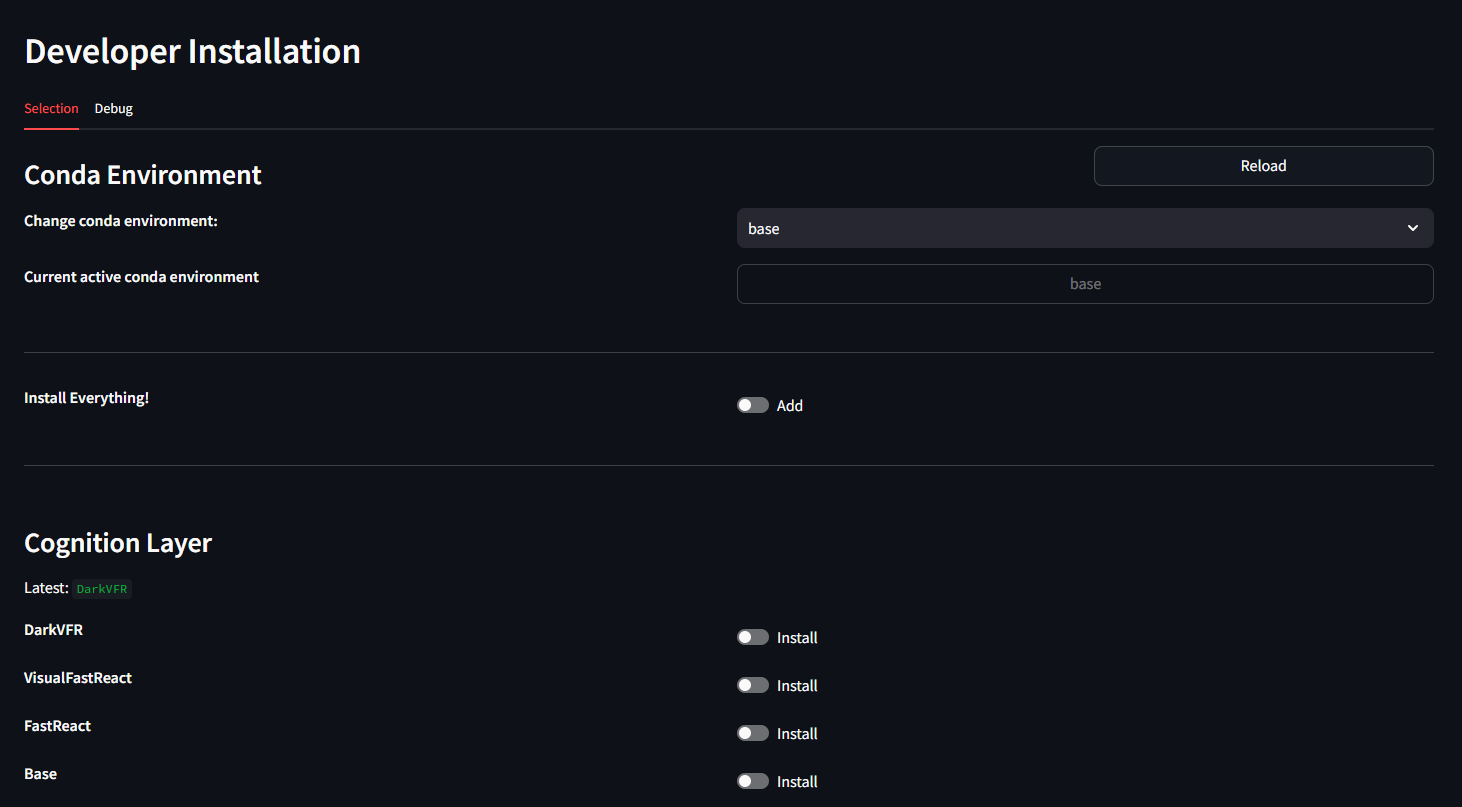
\includegraphics[scale=0.2]{figs/installer.png}
	\caption{\small Interfaz gráfica de desarrollador. Fuente: elaboración propia.}
	\label{fig:installer}
\end{figure}

Este instalador ha sido desarrollado en Python y utiliza la librería
\texttt{streamlit} para la creación de la interfaz gráfica. A su vez, el 
instalador esta envuelto en dos scripts, uno para Windows y otro para
Linux, que permiten la ejecución del instalador sin necesidad
de instalar ninguna dependencia más allá de tener Python3 instalado en
la máquina.

\subsection{Imagen y Kernel para Sistemas Embebidos}
Con el fin de poder integrar la MCE en un sistema embebido, 
(donde la MCE se ejecuta como maestro en el sistema embebido
y la máquina esclava es un dispositivo externo) se ha desarrollado
una imagen de sistema y un bootloader personalizado.

Ambas imagenes han sido desarrolladas desde la placa de desarrollo
IMX8MP de NXP, con un microprocesador ARM Cortex A53 de 4 núcleos. No
se asegura que estas imagenes sean compatibles en su totalidad con otros 
sistemas embebidos, sin embargo, se ha realizado un esfuerzo para que
esta imagen sea lo más portable posible y pueda ser utilizada en otros
entornos.

\subsubsection{Kernel Personalizado}

Usando el repositorio \textit{linux-imx} de \cite{nxp-imx-linux}
como base. Se ha compilado un kernel personalizado que contiene
los requisitos mínimos necesarios para la ejecución de la MCE.

Concretamente, en este kernel se han incluido los drivers necesarios
para la comunicación con la máquina esclava a través de MarvellWifi;
arquitectura de red estandar para comunicaciones a traves de, por ejemplo,
el chipset 88W8997 de Marvell.

A su vez, se han generado los headers necesarios para la compilación
de drivers adicionales que puedan ser necesarios en el futuro.

Junto a este kernel, se ha generado un DTB (Device Tree Blob) que
describe la configuración del hardware del sistema embebido y permite
que el kernel reconozca y utilice correctamente los dispositivos
conectados.

Finalmente, se ha generado fichero \texttt{extlinux.conf} que permite
configurar el arranque del sistema y seleccionar el root filesystem
a utilizar.

\subsubsection{Imagen del Sistema}
La imagen del sistema ha sido generada a partir de la distribución
\emph{Arch Linux ARM} y contiene los siguientes componentes ya instalados:

\begin{itemize}
    \item \textbf{Python 3}: El lenguaje de programación utilizado para la MCE,
    así como todas las dependencias necesarias para su ejecución.
    \item \textbf{Drivers de Red}: Los drivers necesarios para la comunicación
    con la máquina esclava a través de MarvellWifi.
    \item \textbf{Herramientas de Desarrollo}: Herramientas como \texttt{git}, \texttt{make},
    \texttt{gcc} y \texttt{btop} para la gestión del sistema y desarrollo de la MCE.
    \item \textbf{Arranque Automático}: Se ha configurado el sistema para que la MCE se 
    pueda arrancar automáticamente al inicio del sistema gracias a un servicio de systemd.
    \item \textbf{Configuración básica de Seguridad}: Se ha configurado el sistema para 
    que la MCE se ejecute con un usuario específico y se han deshabilitado
    los servicios innecesarios para minimizar los riesgos de posibles ataques.
\end{itemize}

Nótese como a esta imágen no se le ha integrado una interfaz gráfica o gestor de ventanas, 
pues esta solo es necesaria en la máquina esclava, donde se ejecutarán las acciones del espacio 
de acciones \(\mathbb{B}^*\).

\subsubsection{Integración de Kernel e Imagen del Sistema}
Para integrar el kernel y la imagen del sistema, basta con crear
dos particiones en la tarjeta SD del sistema embebido:

\begin{itemize}
    \item \textbf{Partición de arranque}: Esta partición contendrá la imagen del kernel personalizado,
    el DTB y el fichero \texttt{extlinux.conf}.
    \item \textbf{Partición raíz}: Esta partición contendrá la imagen del
    sistema operativo.
\end{itemize}

Es importante revisar que el bootloader este configurado para arrancar
el kernel desde la partición de arranque. Este bootloader generalmente
se encuentra en el comienzo de la memoria de la tarjeta SD y esta
disponible en la documentación del sistema embebido.

\subsection{Integración Continua}
Utilizando las librerías \texttt{pre-commit} y \texttt{pytest} se ha generado
un set de pruebas automatizadas que permite verificar el correcto
funcionamiento de la MCE y sus componentes. 

Estas pruebas son ejecutadas automáticamente cada vez que se realiza un commit
en el repositorio de la MCE, permitiendo verificar que los cambios realizados
no rompen ninguna funcionalidad existente.

Entre los tests automáticos se encuentran:
\begin{itemize}

    \item \textbf{Test Unitarios}: Estos tests verifican el correcto funcionamiento
    de mecanismos independientes como el registro de entidades, el interprete, etc.

    \item \textbf{Test de Integración}: Estos tests verifican que los distintos
    componentes de la MCE funcionan correctamente juntos. Por ejemplo, se verifica
    que el interprete puede cargar acciones desde el registro de entidades y ejecutarlas

    \item \textbf{Bootstraps}: Estos tests pueden ser ejecutados manualmente y verifican
    que la MCE puede ser arrancada correctamente, utilizando distintos compoentes y 
    configuraciones.

    \item \textbf{Tests del espacio de acciones \(\mathbb{B}^*\)}: Estos tests verifican 
    que las acciones del espacio de acciones son realmente ejecutadas en la máquina local y/o 
    máquina esclava y que modifican el entorno de forma correcta.

\end{itemize}

Adicionalmente, se ha configurado el sistema de pre-commit para que
realice un proceso de formateo y revisión de código antes de realizar un commit.
Esto permite mantener un código limpio y legible, así como evitar errores comunes
de sintaxis o estilo.
